%\subsection{5G Architecture} 
%\label{sub:5g_arch}

\begin{figure}[t]
 \centering
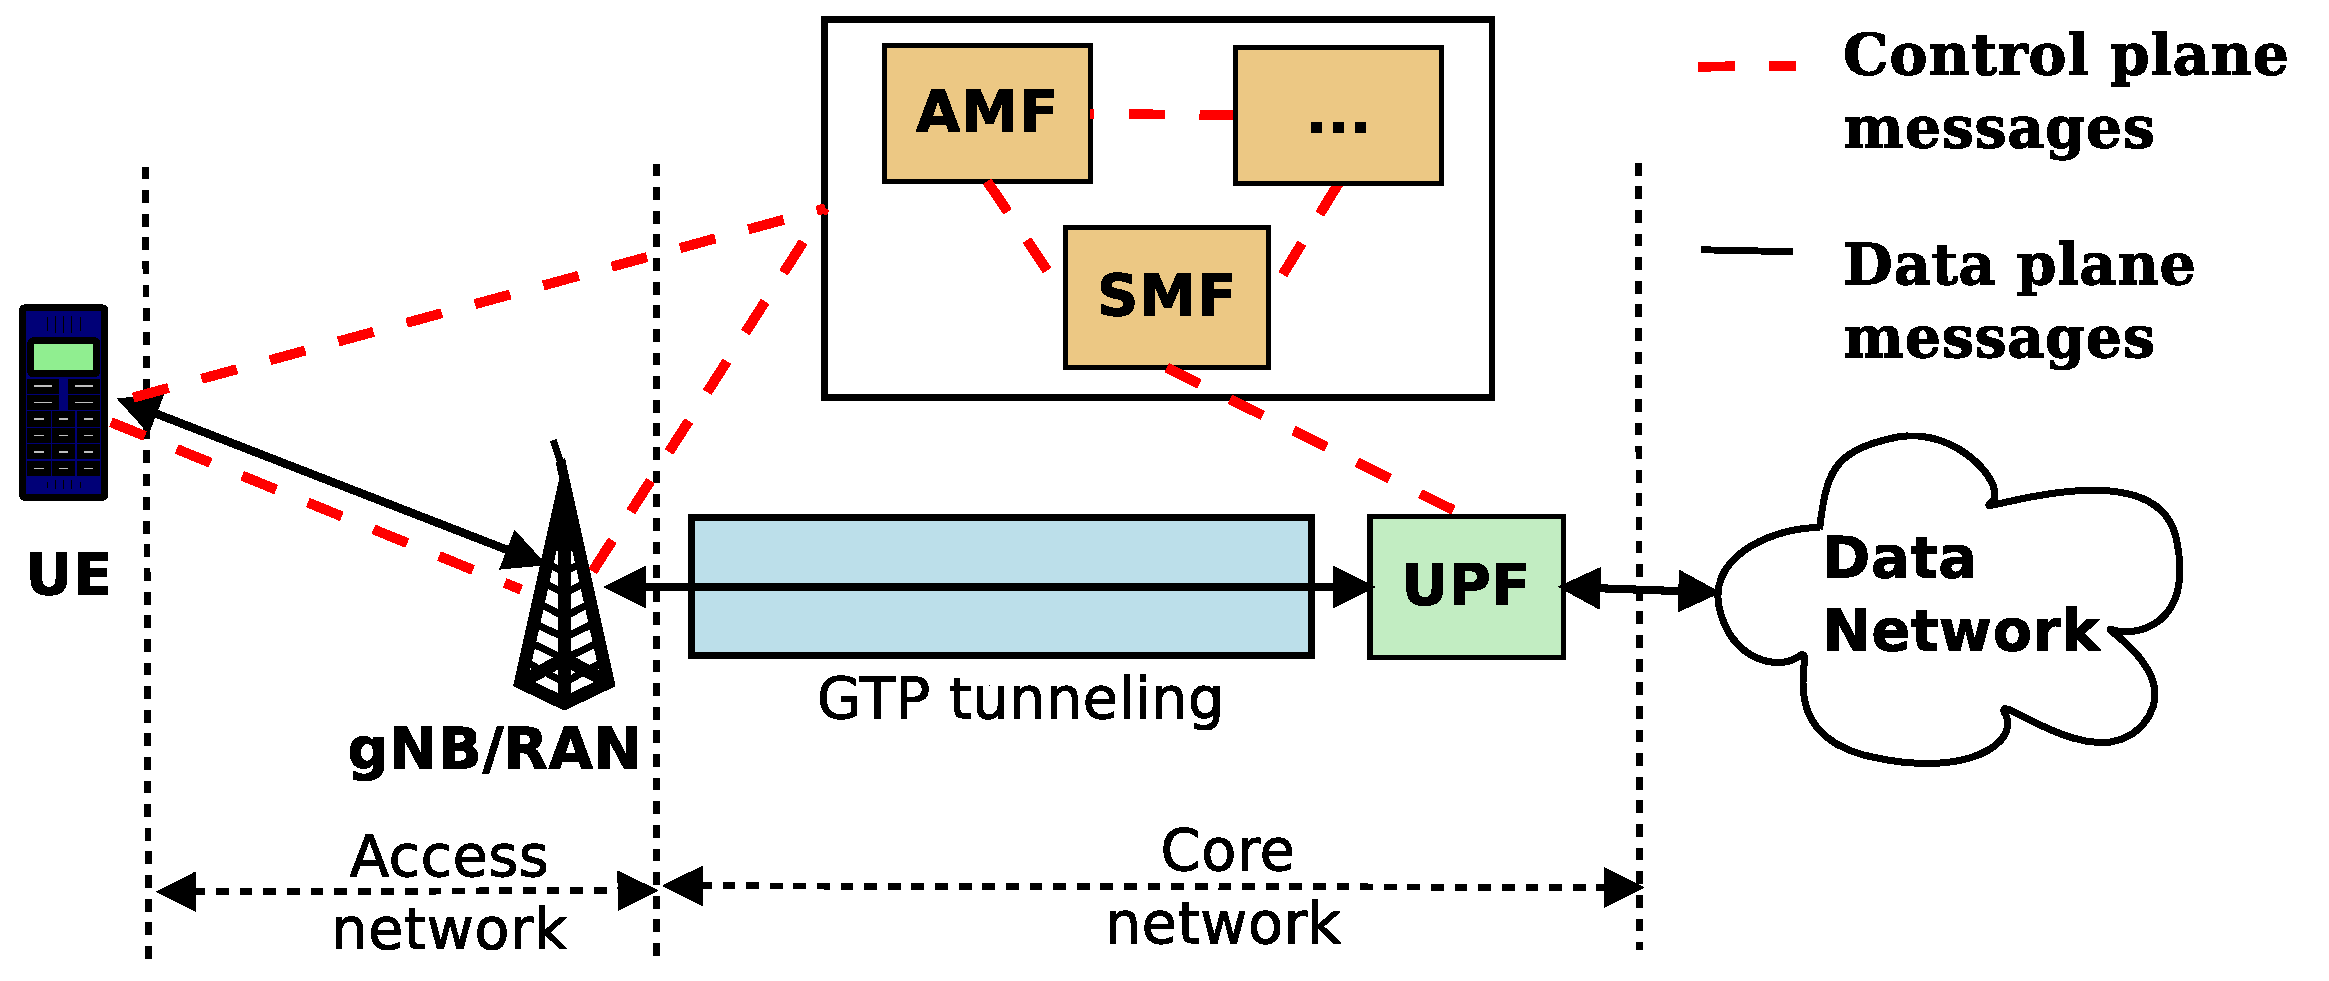
\includegraphics[width=0.4\textwidth]{fig/5g_arch.eps}
%  \setlength{\abovecaptionskip}{-2pt}
\setlength{\belowcaptionskip}{-12pt}
 \caption{5G Architecture.}
 \label{fig:5g_arch}
\end{figure}
%\vspace{-5mm}

\noindent {\bf 5G architecture.} Figure~\ref{fig:5g_arch} shows a high-level overview of the 5G architecture~\cite{5g23501}. A 5G network consists of the wireless radio access network (RAN), which includes the User Equipment (UE) and the Base Station/g-NodeB (gNB), and the wired packet core network. In the control plane of the 5G core, the Access and Mobility Function (AMF) deals with registration and mobility management, and the Session Management Function (SMF) manages the UE's data sessions. The data plane comprises of one or more User Plane Functions (UPFs) that forward user data through the packet core. The control and data plane components communicate using Packet Forwarding Control Protocol (PFCP) messages that are exchanged between the SMF and UPF over UDP~\cite{5g29244}. In the dataplane, a UE's IP datagram packets are encapsulated in GPRS Tunnelling Protocol (GTP) headers when transiting through the packet core; tunnelling aids easy mobility among other things. The GTP-encapsulated IP datagrams are transmitted over a UDP link between the gNB and the UPF. The UPF is responsible for encapsulating downlink packets entering the core with GTP headers and correspondingly decapsulating uplink packets leaving the core. The UPF is also responsible for usage reporting and charging, and enforcing Quality-of-service (QoS), e.g., via rate limiting. 

This paper deals with UPF implementation, so we describe the internal state and data structures at the UPF in more detail. A UE sets up one or more ``sessions'' to forward data through the core, and each data session will cause the SMF to install one or more Packet Detection Rules (PDRs) at the UPF via PFCP messages. A PDR helps associate an incoming data packet to a session based on its GTP/IP packet headers. A PDR has several types of actions associated with it, that instruct the UPF on how to handle the packet. For example, the Forward Action Rules (FARs) specify the forwarding behavior of the packet (e.g., GTP tunnel identifiers for encap), and the QoS Enforcement Rules (QERs) specify the QoS processing to be performed. An example of a field in the QER is the  Aggregate Maximum Bit-Rate (AMBR) of the session. On receiving a PFCP message from the SMF, the UPF creates/updates the required rules, and sends an acknowledgement back to the SMF. On receiving a data packet, the UPF first identifies the matching PDR. For packets belonging to a valid session, the UPF executes forwarding and QoS behavior specified by the FARs and QERs linked to that PDR, in addition to updating usage and charging counters. Packets belonging to ``oversubscribed'' sessions that exceed the rate limit specified in the QoS rules are buffered for an appropriate duration, and scheduled for transmission suitably. 

%%%% Mythili: not sure if we need this figure, can include if there is space.

%Figure~\ref{fig:UPF_DP_proc} shows a simplified data packet processing pipeline in the UPF. 
%
%\begin{figure}[ht]
% \centering
%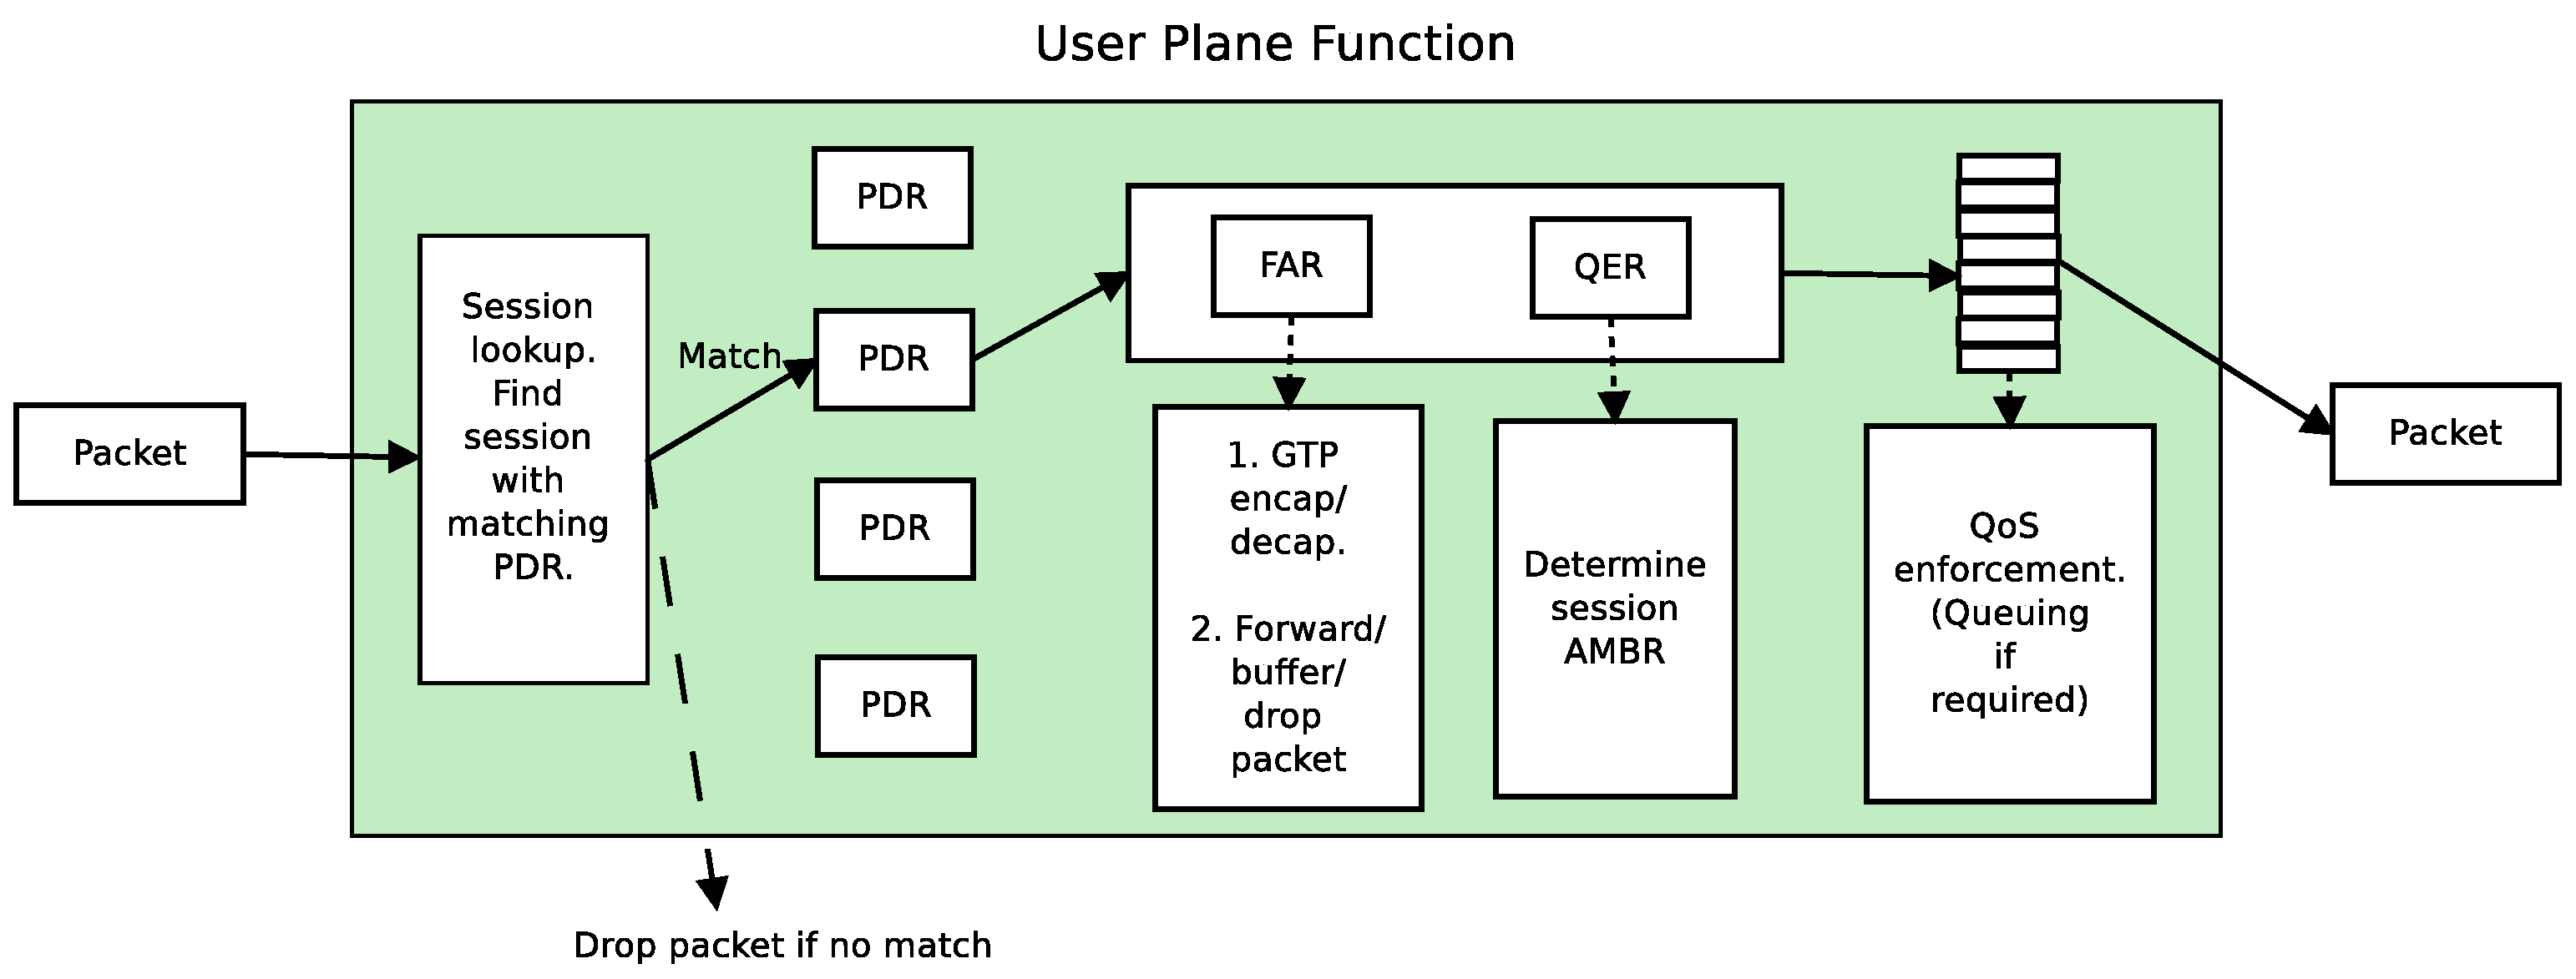
\includegraphics[width=0.5\textwidth]{fig/UPF_DP_processing.eps}
% \setlength{\abovecaptionskip}{6pt}
%% \setlength{\belowcaptionskip}{-6pt}
% \caption{UPF Data Packet processing pipeline.}
% \label{fig:UPF_DP_proc}
%\end{figure}

%%% content below can be deleted after checking once

%
%\noindent \textbf{UPF Data Plane Processing:}
%Fig. \ref{fig:UPF_DP_proc} shows a simplified data packet processing pipeline in the UPF. For each incoming data packet, the UPF browses the existing rules and tries to match the packet against any 1 of the PDRs, based on the packet header fields. If no rule is matched, the UPF discards the packet. If a PDR is matched, it points to the necessary FAR and QER. The UPF may decide whether to forward, buffer or drop the packet, as well as add or remove certain headers based on the FAR. The QER instructs the UPF to enforce necessary QoS. For instance, when a GTP encapsulated data packet for a particular UE arrives at the UPF and a PDR is matched based on the GTP and inner IP header, it will refer to a specific FAR and QER. The FAR may tell the UPF to remove the GTP and outer IP/UDP headers and forward the packet to the DNN. On the other hand, the QER will tell that the UPF should forward packets from that UE at a rate no higher than the specified Aggregate Maximum Bit-Rate (AMBR). To enforce QoS and queue oversubscribed flows in our UPFs, we have implemented the algorithm mentioned in Carousel \cite{carousel} (lines of code: $~XX$) .\\
%% \subsection{P4-SDN-SmartNIC}


%\subsection{State-of-the-art UPFs}

%There are several UPF solutions available today which achieve high performance either by using specialized processing pipelines in s/w or by offloading part of the UPF Data Plane functionalities in the h/w. SK Telecom \cite{intel_wp} uses a SmartNIC to redirect packets to different cores based on Deep Packet Inspection (DPI). 
%% Mavenir \cite{mavenir} compares purely s/w based UPF, UPF with only RSS offloaded, and UPF with both RSS and GTP encapsulation/decapsulation to the h/w in terms of computing costs. 
%Astri \cite{astri} uses Dynamic Device Personalization (DDP) to process packets in the NIC. 
%% Kaloom offloads \cite{kaloom_wp} the Data Plane in h/w. 
%Metaswitch \cite{metaswitch} uses a specilized processing engine (CNAP) in the s/w itself to achive high throughput. However, our work is slightly different from all of the above. We start from a purely s/w based approach and offload the UPF functionalities one by one, comparing the pros ans cons of each design using various metrics. For example, we compare QoS provided, cost per unit of programmable h/w etc. along with regular metrics of throughput and latency in both the Control and the Data Plane. We also propose solutions where queueing in the Data Plane and PFCP parsing in the Control Plane are also offloaded to the h/w.
%
%% \begin{itemize}
%%     \item Intel Whitepaper -- only RSS in h/w
%%     \item Mavenir, APNet-17 -- GTP encap/decap
%%     \item Metaswitch -- P4/gRPC in s/w
%\textbf{[EDIT: Add O-RAN/MEC related work?]}
%% \end{itemize}
